
\section{Ogre3D}
OGRE (Object-Oriented Graphics Rendering Engine) è un motore grafico open-source 3D che essenzialmente offre un'API che sfrutta l'accelerazione hardware per la creazione di applicazioni grafiche. \\

\begin{figure}
\centering
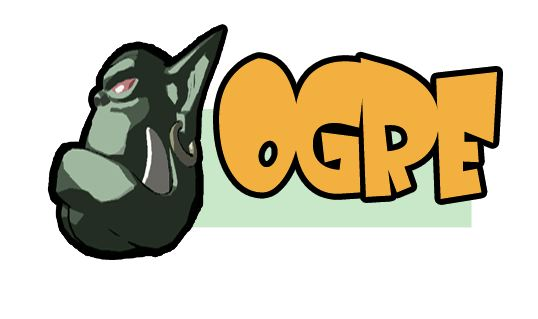
\includegraphics[width=0.6\textwidth]{images/ogre/ogrelogo-small.jpg}

\end{figure}

\subsection{Storia}
E' stato ideato nel 1999 da uno sviluppatore inglese di nome Steve Streeting, dopo che ebbe creato un progetto chiamato "DIMClass", il quale aveva lo scopo di rendere più semplice l'utilizzo della libreria Direct3D. Si rese conto che il livello di astrazione raggiunto dalla sua libreria era cosi elevato che non aveva più bisogno di essere basata su Direct3D. Da qui nacque l'idea di creare una librearia che fosse indipendente da API \cite{ogre-wiki}.

Nel 2000 fu il progetto fu registrato su SourceForge \footnote{ Piattaforma web per portare avanti progetti e software, facilitando la collaborazione tra sviluppatori } registrato il nuovo progetto dalla Sourceforge, con il nome di OGRE. Il 25 febbraio 2005 fu rilasciata la  prima versione di Ogre, la 1.0.0, con il nome di "Azathoth". La versione utilizzata in questo progetto è la 1.9.0, rilasciata il 24 novembre 2013, con il nome "Ghadamon".

\subsection{Il funzionamento di Ogre3D}
Questo framework è scritto in C++ e, a differenza di API quali OpenGL, permette di astrarre tutta la parte a basso livello che invece deve essere implementata negli altri casi.

Utilizza una struttura dati ad albero (scene graph), dove ogni nodo può avere più figli ma un solo padre. Partendo dalla radice, che permette di configurare il sistema, si possono poi creare dei figli per gestire tutta la scena. Il nodo principale è lo "Scene Manager" che, come dice il nome, gestisce tutto ciò che è presente nella scena, come telecamere, oggetti, luci, etc. Solitamente si utilizza un solo Scene Manager, ma è sempre possibile crearne di altri, magari in applicazioni più complesse, per gestire più scene. Questo può essere utilizzato ad esempio per suddividere la finestra in più parti, ognuna delle quali riprende una zona diversa della scena (il cosiddetto split screen).

Dallo Scene Manager è possibile appendere dei nodi chiamati Scene Node, che permettono di gestire più elementi della scena, come entità (i modelli), luci, telecamere, etc. In questo modo è possibile applicare trasformazioni ed effetti a gruppi di oggetti, invece che a ciascuno preso singolarmente.

Infine troviamo i singoli oggetti. Tra questi, come è stato già detto, vi sono i modelli, che vengono rappresentati da oggetti chiamati Entity, i quali devono essere imparentati ad almeno uno Scene Node, tramite il quale sono gestiti. In Ogre, a differenza di OpenGL che richiede una descrizione delle primitive, è possibile creare già dei modelli preimpostati, come ad esempio cubi o piani, oppure possono essere importati dall'esterno.
Inoltre Ogre permette di definire le luci e le telecamere come se fossero oggetti.

Da quello che abbiamo visto notiamo delle semplificazioni. Per esempio quando in OpenGL si importavano modelli esterni, questi dovevano essere prima processati, salvando nei buffer tutti i vertici e altre informazioni quali normali o coordinate uv per le texture, richiedendo diverse righe di codice.
In Ogre invece sono presenti metodi già implementati che, grazie a pochissime righe di codice, permettono di importare modelli sotto forma di file con estensione ".mesh".

Inoltre in OpenGL la gestione di texture, ombre e materiali va implementata a mano scrivendo gli algoritmi di "shading", che contengono informazioni quali il colore o regole di comportamento in presenza di luce. Al contrario in Ogre la gestione di questi aspetti è quasi automatica in quanto di default vengono utilizzati shader già presenti nel framework.

Tuttavia, Ogre è anche versatile perchè lascia all'utente ampie libertà, permettendogli di personalizzare diversi aspetti. Ad esempio in Ogre la view matrix e la perspective matrix, che servono a definire la telecamera, sono generate in automatico, in modo trasparente al programmatore. Poichè la nostra trasformazione richiedeva che le due matrici fossero in funzione della posizione dell'utente, esse sono state calcolate in una funzioni scritte a mano, e poi passate come parametro a due metodi che impostano le trasformazioni a partire da matrici personalizzate.

Inoltre è sempre possibile utilizzare shader personalizzati, e definire i materiali degli oggetti in file con estensione .material, scritti con un linguaggio di facile comprensione, proprio di Ogre.

Per questo, una volta compresa la trasformazione che richiedeva il nostro progetto, è stata abbandonata l'idea di utilizzare OpenGL passando invece a Ogre3D, con lo scopo di concentrarci sulla qualità e la miglior resa della scena.
